%===============================================================================
% LaTeX sjabloon voor de bachelorproef toegepaste informatica aan HOGENT
% Meer info op https://github.com/HoGentTIN/latex-hogent-report
%===============================================================================

\documentclass[dutch,dit,thesis]{hogentreport}

% TODO:
% - If necessary, replace the option `dit`' with your own department!
%   Valid entries are dbo, dbt, dgz, dit, dlo, dog, dsa, soa
% - If you write your thesis in English (remark: only possible after getting
%   explicit approval!), remove the option "dutch," or replace with "english".


%% Pictures to include in the text can be put in the graphics/ folder
\graphicspath{{../graphics/}}

%% For source code highlighting, requires pygments to be installed
%% Compile with the -shell-escape flag!
%% \usepackage[chapter]{minted}
%% If you compile with the make_thesis.{bat,sh} script, use the following
%% import instead:
\usepackage[chapter,outputdir=../output]{minted}
\usemintedstyle{solarized-light}

%% Formatting for minted environments.
%% Code is left-aligned in the sources, so autogobble is unnecessary. Minted
%% 2 in the school container otherwise calls the absent `python` alias.
\setminted{%
    frame=lines,
    breaklines,
    linenos,
    tabsize=4
}

%% Ensure the list of listings is in the table of contents
\renewcommand\listoflistingscaption{%
    \IfLanguageName{dutch}{Lijst van codefragmenten}{List of listings}
}
\renewcommand\listingscaption{%
    \IfLanguageName{dutch}{Codefragment}{Listing}
}
\renewcommand*\listoflistings{%
    \cleardoublepage\phantomsection\addcontentsline{toc}{chapter}{\listoflistingscaption}%
    \listof{listing}{\listoflistingscaption}%
}

% Other packages not already included can be imported here

%%---------- Document metadata -------------------------------------------------
% TODO: Replace this with your own information
\author{Wouter Vantienen}
\supervisor{Ferre De Belie}
%\cosupervisor{Mevr. S. Beeckman}
\title{%
    \texorpdfstring{Real-time detectie van\\personendichtheid op de\\Gentse Feesten via beeldanalyse}%
    {Real-time detectie van personendichtheid op de Gentse Feesten via beeldanalyse}%
}
\academicyear{\advance\year by -1 \the\year--\advance\year by 1 \the\year}
\examperiod{3}
\degreesought{\IfLanguageName{dutch}{Professionele bachelor in de toegepaste informatica}{Bachelor of applied computer science}}
\partialthesis{false} %% To display 'in partial fulfilment'
%\institution{Internshipcompany BVBA.}

%% Add global exceptions to the hyphenation here
\hyphenation{back-slash}

%% The bibliography (style and settings are  found in hogentthesis.cls)
\addbibresource{bachproef.bib}            %% Bibliography file
\addbibresource{../voorstel/voorstel.bib} %% Bibliography research proposal
\defbibheading{bibempty}{}

%% Prevent empty pages for right-handed chapter starts in twoside mode
\renewcommand{\cleardoublepage}{\clearpage}

\renewcommand{\arraystretch}{1.2}

%% Content starts here.
\begin{document}

%---------- Front matter -------------------------------------------------------

\frontmatter

\hypersetup{pageanchor=false} %% Disable page numbering references
%% Render a Dutch outer title page if the main language is English
\IfLanguageName{english}{%
    %% If necessary, information can be changed here
    \degreesought{Professionele Bachelor toegepaste informatica}%
    \begin{otherlanguage}{dutch}%
       \maketitle%
    \end{otherlanguage}%
}{}

%% Generates title page content
\maketitle
\hypersetup{pageanchor=true}

%%=============================================================================
%% Voorwoord
%%=============================================================================

\chapter*{\IfLanguageName{dutch}{Woord vooraf}{Preface}}%
\label{ch:voorwoord}

Deze bachelorproef vormt het sluitstuk van de opleiding Toegepaste Informatica aan HOGENT. Het onderwerp combineert twee domeinen die mij bijzonder interesseren: de praktische inzet van artificiële intelligentie en de veilige organisatie van drukbezochte evenementen. De Gentse Feesten bieden daarbij een herkenbare en maatschappelijk relevante casus.

Ik dank mijn promotor, Ferre De Belie, voor de begeleiding, kritische vragen en feedback tijdens dit traject. Daarnaast dank ik iedereen die mij met technische of inhoudelijke feedback heeft geholpen en mij de ruimte gaf om aan deze bachelorproef te werken.

%%=============================================================================
%% Samenvatting
%%=============================================================================

\chapter*{\IfLanguageName{dutch}{Samenvatting}{Abstract}}

De Gentse Feesten brengen gedurende tien dagen grote en voortdurend veranderende bezoekersstromen naar de Gentse binnenstad. Voor organisatoren en hulpdiensten is een algemeen bezoekersaantal onvoldoende: zij hebben vooral nood aan een actueel beeld van lokale drukte. Het handmatig interpreteren van meerdere camerabeelden is echter arbeidsintensief. Deze bachelorproef onderzoekt daarom hoe computervisie, meer bepaald \emph{density estimation}, een aanvullende indicatie van lokale drukte kan leveren.

Er werd een literatuurstudie uitgevoerd naar crowd management, bestaande methoden voor druktemeting en computervisie voor crowd counting. Op basis daarvan werd CSRNet gekozen als reproduceerbare eerste baseline. De Proof of Concept zet de puntannotaties van ShanghaiTech Part B om naar density maps, traint een CSRNet-model met een voorgetrainde VGG-16-frontend en evalueert de volledige validatiebeelden met MAE en RMSE. Van de officiële trainingsset worden met een vaste seed 360 beelden voor training en 40 beelden voor validatie gebruikt. De officiële testset werd niet gebruikt voor modelselectie.

Na technische kalibraties werd een deterministische GPU-run van 100 epochs uitgevoerd. Het checkpoint met de laagste validatie-MAE ligt op epoch 39 en behaalt een MAE van \(6{,}556\) personen, een RMSE van \(9{,}218\) personen en een gemiddelde getekende fout van \(-0{,}304\) personen. Tegenover een gecontroleerde run van één epoch met dezelfde finale configuratie dalen MAE en RMSE respectievelijk met \(76{,}5\%\) en \(77{,}4\%\). Voor een beeld van \(1024 \times 768\) pixels duurt uitsluitend de model-inferentie op de RTX 3050 Ti gemiddeld \(107\) ms, of 9,3 model-doorlopen per seconde. Op de CPU van een Raspberry Pi 5 bedraagt dit \(10{,}95\) s per beeld, of 0,091 FPS, waarbij tijdens de belasting thermische throttling optrad. De volledige trainingsrun duurt \(58{,}19\) minuten. De resultaten tonen aan dat de technische keten reproduceerbaar werkt en dat modelselectie op volledige validatiebeelden noodzakelijk is.

De PoC schat een aantal personen en een relatieve verdeling in beeldcoördinaten. Zonder camerakalibratie en projectie naar het grondvlak kan een density map niet worden vertaald naar personen per vierkante meter en kan zij geen zelfstandige veiligheidsdrempel activeren. Bovendien vereist een reële uitrol representatieve beelden van de Gentse Feesten, een evaluatie van de volledige verwerkingsketen en een privacy- en gegevensbeschermingsanalyse. De PoC is daarom bedoeld als beslissingsondersteunende basis voor verder onderzoek, niet als een onmiddellijk inzetbaar alarmsysteem.


%---------- Inhoud, lijst figuren, ... -----------------------------------------

\tableofcontents

% In a list of figures, the complete caption will be included. To prevent this,
% ALWAYS add a short description in the caption!
%
%  \caption[short description]{elaborate description}
%
% If you do, only the short description will be used in the list of figures

\listoffigures

% If you included tables and/or source code listings, uncomment the appropriate
% lines.
\listoftables

\listoflistings

% Als je een lijst van afkortingen of termen wil toevoegen, dan hoort die
% hier thuis. Gebruik bijvoorbeeld de ``glossaries'' package.
% https://www.overleaf.com/learn/latex/Glossaries

%---------- Kern ---------------------------------------------------------------

\mainmatter{}

% De eerste hoofdstukken van een bachelorproef zijn meestal een inleiding op
% het onderwerp, literatuurstudie en verantwoording methodologie.
% Aarzel niet om een meer beschrijvende titel aan deze hoofdstukken te geven of
% om bijvoorbeeld de inleiding en/of stand van zaken over meerdere hoofdstukken
% te verspreiden!

%%=============================================================================
%% Inleiding
%%=============================================================================

\chapter{\IfLanguageName{dutch}{Inleiding}{Introduction}}%
\label{ch:inleiding}

Tijdens de Gentse Feesten verplaatsen grote groepen bezoekers zich voortdurend tussen pleinen, straten en podia. De drukte is daardoor niet gelijkmatig over de binnenstad verdeeld: een locatie kan in korte tijd vollopen, terwijl het elders relatief rustig blijft. Voor hulpdiensten is het daarom niet alleen relevant hoeveel bezoekers op het evenement aanwezig zijn, maar vooral waar de drukte toeneemt, hoe snel dat gebeurt en welke doorgangen daarbij onder druk komen te staan. Recente veiligheidsmaatregelen, zoals het spreiden van de uitstroom na een bijzonder drukke feestendag, illustreren de nood aan een actueel beeld van bezoekersstromen \autocite{Aneca2024}.

Camera's kunnen lokale veranderingen continu zichtbaar maken, maar het gelijktijdig beoordelen van meerdere videobeelden blijft arbeidsintensief. Computervisie biedt een manier om die beelden automatisch te analyseren. In zeer drukke scènes is het vaak moeilijk om elke persoon afzonderlijk te detecteren, bijvoorbeeld door overlap, perspectiefverschillen en wisselende belichting. Daarom onderzoekt deze bachelorproef \emph{density estimation}: een techniek die een dichtheidskaart voorspelt waarvan de som een schatting geeft van het aantal personen in beeld \autocite{Khan2020}. Zo'n kaart kan drukke zones zichtbaar maken en hulpdiensten van aanvullende, objectieve informatie voorzien.

\section{\IfLanguageName{dutch}{Probleemstelling}{Problem Statement}}%
\label{sec:probleemstelling}

De Gentse Feesten vinden sinds 1843 plaats en groeiden uit tot een tiendaags cultureel volksfeest in de historische binnenstad. In 2023 werden meer dan 1,6 miljoen bezoekers geteld, verspreid over dag en nacht \autocite{StadGentGeschiedenis}. Omdat het evenement niet op één afgesloten terrein plaatsvindt, verplaatsen bezoekers zich vrij tussen locaties. Een algemeen bezoekersaantal zegt daardoor weinig over lokale drukte of mogelijke knelpunten.

Een hoge personendichtheid kan de bewegingsvrijheid beperken en het risico op gevaarlijke situaties verhogen. Organisatoren en hulpdiensten baseren zich daarvoor onder meer op terreinobservaties, handmatige tellingen en ervaring uit voorgaande edities. Die werkwijze blijft onmisbaar, maar kan niet gelijktijdig elke locatie opvolgen en leidt onvermijdelijk tot een vertraging tussen waarnemen, afstemmen en handelen.

Stad Gent experimenteerde reeds met meerdere vormen van druktemeting. Het project VLOED wijst op de nood aan fijnmazige, actuele informatie over de ruimtelijke spreiding van drukte \autocite{StadGentVloed}. Er is echter een bijkomende vertaalslag nodig om camerabeelden om te zetten in informatie die operationeel bruikbaar is. Dit onderzoek verkent in welke mate een density-estimationmodel daarvoor een technische basis kan vormen.

\section{\IfLanguageName{dutch}{Onderzoeksvraag}{Research question}}%
\label{sec:onderzoeksvraag}

Hoe kan computervisie, meer bepaald density estimation, bruikbare en tijdige indicaties van lokale drukte leveren tijdens openluchtevenementen zoals de Gentse Feesten?

\textit{Deelvragen rond het probleemdomein:}
\begin{itemize}
    \item Welke factoren maken lokale drukte risicovol, en welke informatie hebben hulpdiensten nodig om proactief te kunnen ingrijpen?
    \item Welke bestaande technieken voor druktemeting zijn beschikbaar en welke beperkingen hebben ze voor een verspreid stadsfestival?
\end{itemize}

\textit{Deelvragen rond het oplossingsdomein:}
\begin{itemize}
    \item Waarom is density estimation een geschikte aanvulling op persoonsdetectie in dicht bezette scènes?
    \item Welke dataset, evaluatiemetrieken en experimentele opzet zijn nodig om een eerste model reproduceerbaar te beoordelen?
    \item Welke nauwkeurigheid en inferentiesnelheid bereikt een CSRNet-baseline op ShanghaiTech Part B?
    \item Welke bijkomende kalibratie is nodig om een dichtheidskaart in beeldcoördinaten te vertalen naar een fysieke dichtheid in personen per vierkante meter?
\end{itemize}

\section{\IfLanguageName{dutch}{Onderzoeksdoelstelling}{Research objective}}%
\label{sec:onderzoeksdoelstelling}

Het doel van dit onderzoek is een reproduceerbare Proof of Concept (PoC) te realiseren die met CSRNet een density map en een geschat aantal personen uit één camerabeeld afleidt. De PoC wordt geëvalueerd op ShanghaiTech Part B aan de hand van de Mean Absolute Error (MAE), de Root Mean Squared Error (RMSE) en de gemeten inferentietijd. De resultaten tonen welke prestaties een eerste baseline haalt en welke stappen nog nodig zijn voor inzet in de context van de Gentse Feesten.

De PoC is beslissingsondersteunend: zij kan een operator attenderen op relatieve veranderingen of drukke zones, maar vervangt geen menselijke beoordeling. De dichtheidskaart drukt in de huidige opzet een verdeling in beeldpixels uit. Ze kan dus niet zonder camerakalibratie worden geïnterpreteerd als een fysieke dichtheid in personen per vierkante meter, en vormt op zichzelf geen grond voor een veiligheidsalarm. Het onderzoek richt zich evenmin op het herkennen of volgen van individuele bezoekers.

\section{\IfLanguageName{dutch}{Opzet van deze bachelorproef}{Structure of this bachelor thesis}}%
\label{sec:opzet-bachelorproef}

Hoofdstuk~\ref{ch:stand-van-zaken} situeert de Gentse Feesten als casus, bespreekt risico's en bestaande technieken voor druktemeting en motiveert de keuze voor density estimation. Hoofdstuk~\ref{ch:methodologie} beschrijft de onderzoeksmethode, de datasetsplitsing en het evaluatieprotocol.

Hoofdstuk~\ref{ch:poc} licht de implementatie van CSRNet toe en rapporteert de resultaten van de uitgevoerde CPU- en GPU-experimenten. Ten slotte beantwoordt Hoofdstuk~\ref{ch:conclusie} de onderzoeksvraag, plaatst het de resultaten in hun context en formuleert het aanbevelingen voor verder onderzoek en eventuele operationele inzet.

\chapter{\IfLanguageName{dutch}{Stand van zaken}{State of the art}}%
\label{ch:stand-van-zaken}

Dit hoofdstuk situeert de Gentse Feesten als casus voor lokale druktemeting. Eerst worden de veiligheidscontext en de beperkingen van bestaande meetmethoden besproken. Daarna volgt een afbakening van computervisiemethoden, met bijzondere aandacht voor \emph{density estimation}. De bespreking leidt tot de keuze van CSRNet als reproduceerbare eerste baseline.

\section{De Gentse Feesten als casus}

De Gentse Feesten ontstonden in 1843 als centraal georganiseerde Gemeentefeesten. Na een periode van teruglopende belangstelling kregen zij vanaf 1970 een nieuwe impuls rond Sint-Jacobs, onder meer door Walter De Buck en Trefpunt. Sindsdien groeiden de Feesten uit tot een groot cultureel volksfeest dat gedurende tien dagen in de Gentse binnenstad plaatsvindt. In 2021 werden de Gentse Feesten erkend als Vlaams Immaterieel Erfgoed. Tijdens de editie van 2023 werden meer dan 1,6 miljoen bezoekers geteld \autocite{StadGentGeschiedenis}.

In tegenstelling tot een evenement op een afgesloten terrein zijn de Gentse Feesten verspreid over pleinen, straten en binnenlocaties. Bezoekers kunnen zich vrij tussen die locaties verplaatsen en de bezetting verandert voortdurend doorheen de dag en nacht. Het totale bezoekersaantal zegt daarom weinig over de drukte op één specifieke plaats. Wanneer programma's gelijktijdig eindigen of bezoekersstromen samenkomen in smalle straten, kan de lokale bezetting snel toenemen.

Recente edities illustreren dat zulke veranderingen operationele aandacht vragen. Tijdens de openingsavond van 2023 liet de politie tijdelijk geen bijkomende bezoekers toe op Boomtown en het Laurentplein, omdat het er te druk werd \autocite{Schouppe2023}. In 2024 bleven de pleinen uitzonderlijk een uur langer open om een gelijktijdige uitstroom na een bijzonder drukke dag te vermijden \autocite{Aneca2024}. Deze situaties tonen niet noodzakelijk een incident aan, maar wel dat organisatoren soms snel moeten beslissen op basis van veranderende bezoekersstromen.

Stad Gent onderzocht eerder al, samen met onder meer de Universiteit Gent, verschillende vormen van druktemeting. Het project VLOED noemt fijnmazige informatie over de ruimtelijke spreiding van drukte, aangevuld met actuele gegevens en voorspellingen, als belangrijke behoefte \autocite{StadGentVloed}. Een automatische analyse van camerabeelden kan daarop aansluiten, op voorwaarde dat de resultaten begrijpelijk, betrouwbaar en zorgvuldig ingebed zijn in de bestaande besluitvorming.

\section{Risico's bij lokale drukte}

De veiligheid van een menigte hangt niet alleen af van het aantal aanwezigen. Ook de beschikbare ruimte, de vorm van doorgangen, de richting en snelheid van stromen, de duur van de drukte en de communicatie tussen betrokken diensten spelen een rol \autocite{Helbing2000,Zeitz2009,Hutton2025}. Hoge dichtheden kunnen de bewegingsvrijheid sterk beperken; in combinatie met ongunstige omstandigheden kunnen zij tot gevaarlijke druk en verlies van controle over de beweging leiden. Een systeem voor druktemeting moet daarom als vroegtijdige informatiebron worden beschouwd, niet als een zelfstandige voorspeller van incidenten.

Literatuur noemt dichtheden van ongeveer acht tot tien personen per vierkante meter als bijzonder kritisch \autocite{Haghani2022}. Een vaste alarmwaarde kan echter niet rechtstreeks uit een camerabeel of density map worden afgeleid. Daarvoor moet elk beeld eerst via camerakalibratie en een grondvlaktransformatie aan een reële oppervlakte worden gekoppeld. Ook de locatie, de richting van de stroom en de duur van een verhoogde dichtheid moeten in een operationele drempel worden meegenomen. In deze bachelorproef wordt daarom geen veiligheidsdrempel ingesteld; de PoC beperkt zich tot personentellingen en relatieve druktepatronen in beeldcoördinaten.

\section{Bestaande meetmethoden en de rol van automatisering}

Organisatoren combineren vaak terreinobservaties, handmatige tellingen en ervaring uit voorgaande edities. Deze bronnen blijven waardevol, maar zijn niet continu en niet overal tegelijk beschikbaar. Tussen de waarneming, de interpretatie, de communicatie en een eventuele maatregel ontstaat bovendien onvermijdelijk vertraging. Automatische metingen kunnen die menselijke beoordeling aanvullen met een regelmatige en reproduceerbare indicatie van lokale veranderingen.

WiFi- en Bluetoothsignalen kunnen worden gebruikt om personen te tellen of te lokaliseren \autocite{GuillenPerez2019}. Hun ruimtelijke resolutie en nauwkeurigheid hangen echter af van de meetopstelling, de aanwezigheid van apparaten en de gebruikte methode. Camerabeelden bieden in principe een fijnere ruimtelijke observatie van één afgebakende zone, maar stellen eisen aan zichtbaarheid, rekenkracht, privacy en robuustheid tegen variaties in de scène. Computervisie is daarom geen vervanging van andere meetbronnen, maar een mogelijke aanvullende sensor.

\section{Computervisie voor crowd counting}

De meeste moderne methoden voor beeldanalyse gebruiken convolutionele neurale netwerken (CNN's), die visuele patronen uit beelden leren \autocite{OShea2015}. Binnen crowd counting zijn twee uitvoerwijzen relevant. \emph{Objectdetectie} zoekt individuele personen en voorspelt voor elke detectie een begrenzingskader. \emph{Density estimation} voorspelt daarentegen een tweedimensionale kaart waarvan de waarden de lokale aanwezigheid van personen weergeven. Beide benaderingen kunnen CNN's gebruiken; het verschil ligt dus in de taak en de uitvoer, niet in het al dan niet gebruiken van een CNN.

Objectdetectie is aantrekkelijk wanneer personen voldoende zichtbaar en van elkaar te onderscheiden zijn. YOLO is bijvoorbeeld ontworpen voor snelle objectdetectie \autocite{Redmon2016}. In dichte menigtes verminderen overlap, schaalverschillen en gedeeltelijke zichtbaarheid echter de betrouwbaarheid van afzonderlijke detecties \autocite{Khan2020}. Een density-estimationmodel hoeft niet voor elke persoon een afzonderlijk kader te vinden. Het kan daardoor in zulke scènes een bruikbare telling en ruimtelijk patroon leveren, al blijft de nauwkeurigheid afhankelijk van de trainingsdata en de gelijkenis met de doelomgeving.

Een \emph{density map} is geen directe kaart in personen per vierkante meter. De kaart is gekoppeld aan beeldpixels of aan cellen in de uitvoerresolutie van het model. De som van alle waarden levert een geschat aantal personen in het zichtveld. Pas na camerakalibratie en projectie naar het grondvlak kan een dichtheidswaarde aan een fysieke oppervlakte worden gekoppeld.

\section{Selectie van een eerste baseline}

Tabel~\ref{tab:long-list-modellen} vergelijkt kandidaatmodellen op basis van hun hoofdidee, hun sterkte voor deze casus en hun voornaamste beperking. De tabel is geen benchmark: de modellen worden niet onder identieke omstandigheden uitgevoerd. Zij dient uitsluitend om de keuze voor een eerste implementatie te verantwoorden.

\begin{table}[htbp]
    \centering
    \small
    \begin{tabular}{|p{2.4cm}|p{2.6cm}|p{4.2cm}|p{4.1cm}|}
        \hline
        \textbf{Model} & \textbf{Categorie} & \textbf{Relevante sterkte} & \textbf{Beperking voor deze PoC} \\
        \hline
        YOLO \autocite{Redmon2016} & Objectdetectie & Snelle detectie wanneer personen afzonderlijk zichtbaar zijn. & Overlap tussen personen bemoeilijkt afzonderlijke detecties. \\
        \hline
        Faster R-CNN & Objectdetectie & Sterke referentie voor nauwkeurige objectdetectie. & Complexer en doorgaans trager voor een eerste baseline met real-timeambitie. \\
        \hline
        SSD & Objectdetectie & Relatief compacte detector met een bruikbare snelheids-nauwkeurigheidsbalans. & Blijft afhankelijk van afzonderlijke begrenzingskaders. \\
        \hline
        RetinaNet & Objectdetectie & Ontworpen om de onbalans tussen achtergrond en objecten te beperken. & Niet specifiek gericht op zeer dichte menigtes. \\
        \hline
        CSRNet \autocite{Li2018} & Density estimation & Gedilateerde convoluties behouden context en ruimtelijk detail. & Vereist training en validatie voor de doelomgeving. \\
        \hline
        MCNN \autocite{Zhang2016} & Density estimation & Meerdere kolommen behandelen schaal- en perspectiefvariatie. & Oudere en zwaardere architectuur als eerste baseline. \\
        \hline
        SANet & Density estimation & Combineert informatie op verschillende schalen. & Hogere implementatiecomplexiteit. \\
        \hline
        CAN & Density estimation & Gebruikt contextuele informatie voor de dichtheidsschatting. & Hogere complexiteit en minder geschikt voor een minimale baseline. \\
        \hline
    \end{tabular}
    \caption[Selectie van kandidaatmodellen]{Kwalitatieve selectie van kandidaatmodellen voor druktemeting.}
    \label{tab:long-list-modellen}
\end{table}

CSRNet wordt geselecteerd als eerste baseline omdat de architectuur specifiek is ontwikkeld voor dicht bezette scènes, volledig convolutioneel is en goed gedocumenteerd werd op ShanghaiTech \autocite{Li2018}. MCNN blijft een zinvolle referentie voor toekomstig vergelijkend onderzoek, maar wordt binnen de beschikbare scope niet geïmplementeerd. De resultaten in deze bachelorproef mogen bijgevolg niet worden gelezen als een vergelijking tussen modellen.

\section{Privacy en gegevensbescherming}

Density estimation heeft als voordeel dat de PoC geen gezichten herkent, personen heridentificeert of trajecten volgt. Dat beperkt de functionaliteit tot een telling en een ruimtelijk patroon. De camerabeelden kunnen desondanks personen identificeerbaar in beeld brengen en zijn dan persoonsgegevens. Een density-estimationmodel maakt de verwerking dus niet automatisch anoniem of conform de AVG.

Een productie-oplossing vereist minstens een welbepaalde rechtsgrond en doel, dataminimalisatie, transparante informatie voor bezoekers, beperkte bewaartermijnen, toegangscontrole en passende beveiliging. Bij grootschalige monitoring van een publiek toegankelijke ruimte kan bovendien een gegevensbeschermingseffectbeoordeling vereist zijn \autocite{EDPBVideo2020}. Praktische maatregelen, zoals verwerking aan de rand van het netwerk, het niet bewaren van ruwe beelden en het beperken van de analyse tot afgebakende zones, verdienen daarbij verder onderzoek. De PoC evalueert deze maatregelen niet en doet geen uitspraak over juridische conformiteit.

%%=============================================================================
%% Methodologie
%%=============================================================================

\chapter{\IfLanguageName{dutch}{Methodologie}{Methodology}}%
\label{ch:methodologie}

Dit onderzoek combineert een literatuurstudie met een experimentele evaluatie van een reproduceerbare CSRNet-baseline. De literatuurstudie kadert de operationele nood, de technische mogelijkheden en de beperkingen van beeldanalyse. Het experiment toetst vervolgens of de volledige keten --- van puntannotaties tot density map, modeltraining en full-image-evaluatie --- technisch correct werkt. De resultaten zijn bedoeld als baseline en niet als bewijs dat het systeem al inzetbaar is op de Gentse Feesten.

\section{Literatuurstudie en afbakening}

Eerst worden crowd management, bestaande methoden voor druktemeting en computervisiemethoden onderzocht. De recente survey van \textcite{Gao2025} vormt daarbij het vertrekpunt voor density estimation; aanvullende bronnen kaderen de risico's bij massabijeenkomsten en de lokale Gentse context. Op basis hiervan wordt CSRNet geselecteerd als een goed gedocumenteerde baseline voor dichte menigtes. De keuze voor één model maakt een grondige technische validatie mogelijk, maar beperkt de uitspraken over de relatieve prestaties van andere architecturen.

\section{Dataset en voorbereiding}

Voor de eerste experimenten wordt ShanghaiTech Part B gebruikt, een deel van de dataset van \textcite{Zhang2016}. Deze subset bevat 400 officiële trainingsbeelden en 316 officiële testbeelden. Uit de officiële trainingsset worden met seed 42 veertig beelden als vaste validatieset geselecteerd; de resterende 360 beelden vormen de trainingsset. De officiële testset blijft buiten de modelselectie en wordt in deze bachelorproef enkel gebruikt voor een kwalitatieve visualisatie. Daardoor blijven de gerapporteerde MAE en RMSE zuivere validatieresultaten en worden zij niet ten onrechte als testprestaties voorgesteld.

De dataset bevat puntannotaties van hoofden. Voor elk beeld worden die annotaties omgezet naar een density map door op elk punt een Gaussische kernel met een vaste standaardafwijking van vier pixels te plaatsen. De map wordt daarna zo genormaliseerd dat de som van alle pixels exact gelijk is aan het aantal annotaties. Die eigenschap wordt automatisch gecontroleerd. Een vaste kernel levert een reproduceerbare baseline; perspectief- of geometrieafhankelijke kernels zijn mogelijke uitbreidingen.

ShanghaiTech Part B is geschikt om de technische keten te vergelijken met bestaand crowd-countingonderzoek, maar vertegenwoordigt niet de volledige variatie van camerabeelden tijdens de Gentse Feesten. Belichting, camerahoek, weersomstandigheden, lokale architectuur en bezoekersgedrag kunnen tot domeinverschuiving leiden. Een validatie met rechtmatig verkregen, representatieve lokale beelden is daarom noodzakelijk vóór een operationele toepassing.

\section{Training en modelselectie}

CSRNet wordt in Python met PyTorch geïmplementeerd. De ImageNet-voorgetrainde VGG-16-frontend wordt verfijnd voor density estimation; de backend met gedilateerde convoluties voorspelt de density map. Tijdens de training worden willekeurige vierkante uitsneden gebruikt om het geheugengebruik te beperken en beelden in batches te kunnen verwerken. Voor de finale configuratie bedraagt die uitsnede \(512 \times 512\) pixels. Dit is dus geen herschaling van het volledige invoerbeeld. De keuze is een praktisch compromis: tegenover een uitsnede van \(256 \times 256\) pixels krijgt het model meer ruimtelijke context te zien, terwijl vier uitsneden tegelijk op de beschikbare GPU met 4~GB VRAM passen. De cropgrootte is niet via een afzonderlijke hyperparametervergelijking als optimaal bepaald. De validatie verwerkt steeds het volledige beeld, zodat de fout betrekking heeft op de volledige geschatte telling.

Voor elke trainingsrun worden de datasetversie, seed, cropgrootte, batchgrootte, leersnelheid, hardware en resultaten bewaard. Het checkpoint met de laagste validatie-MAE wordt als beste model aangeduid. Daarnaast worden het laatst voltooide checkpoint en periodieke tussentijdse checkpoints opgeslagen. Een hervatte run herstelt ook de optimizer, mixed-precisionstatus en toestand van de toevalsgetallengeneratoren. Dit protocol voorkomt dat configuraties op de officiële testset worden gekozen en maakt de experimenten controleerbaar.

\section{Evaluatiecriteria}

De nauwkeurigheid wordt berekend op de totale telling per volledig validatiebeeld. De MAE geeft de gemiddelde absolute afwijking in aantal personen weer; de RMSE weegt grote afwijkingen zwaarder door. Beide metrieken worden aangevuld met een visuele controle van de voorspelde density maps. Daarbij wordt nagegaan of zones met een hogere voorspelde dichtheid overeenkomen met de geannoteerde drukke zones.

De technische haalbaarheid wordt beoordeeld aan de hand van de gemiddelde tijd voor één voorwaartse modelberekening op een beeld van \(1024 \times 768\) pixels met batchgrootte één. De modeldoorvoer in beelden per seconde wordt berekend als
\[
    \mathrm{FPS}_{\mathrm{model}} = \frac{1000}{\overline{t}_{\mathrm{forward,ms}}}.
\]
Voor de afzonderlijke platformbenchmark worden eerst drie opwarmruns uitgevoerd en daarna twintig voorwaartse berekeningen op hetzelfde beeld gemeten. De vergelijking omvat de laptop-GPU, de laptop-CPU en een Raspberry Pi 5-CPU. Temperatuur- en throttlingstatus worden op de Raspberry Pi voor en na de meetreeks geregistreerd. Deze meting is geen latentie van de volledige verwerkingsketen. Het laden van een videoframe, voor- en nabewerking, visualisatie en netwerkoverdracht vallen er buiten. Een mogelijke eis van 15 beelden per seconde komt neer op maximaal \(66{,}7\) ms per volledig verwerkt frame en moet daarom later op de volledige keten worden gevalideerd.

\section{Beperkingen en ethische randvoorwaarden}

Een density map maakt relatieve drukte in het beeld zichtbaar, maar levert zonder kalibratie geen aantal personen per vierkante meter. Voor fysieke drempelwaarden zijn minstens een grondvlaktransformatie, een afgebakende observatiezone en een procedure om de nauwkeurigheid per camera te controleren nodig. Waarschuwingen mogen daarom pas na zulke kalibratie en in combinatie met menselijke beoordeling worden ontworpen.

De PoC voert geen gezichtsherkenning, heridentificatie of persoonsvolging uit. Toch kunnen camerabeelden persoonsgegevens bevatten. Bij een reële uitrol zijn een duidelijke rechtsgrond, doelbinding, dataminimalisatie, transparantie, beveiliging en een beoordeling van de gegevensbescherming nodig; grootschalige monitoring van publiek toegankelijke ruimten kan een gegevensbeschermingseffectbeoordeling vereisen \autocite{EDPBVideo2020}. Deze juridische en organisatorische uitwerking valt buiten de scope van de PoC.

\section{Gebruik van generatieve artificiële intelligentie}

Bij de ontwikkeling en herwerking van de Pythonbroncode is generatieve artificiële intelligentie gebruikt. Meer bepaald werd OpenAI Codex met het model \mbox{GPT-5.6-sol} van provider OpenAI ingezet om code te genereren en te refactoren, foutmeldingen te analyseren, regressietests op te stellen en documentatie bij de scripts te formuleren. Dezelfde omgeving werd beperkt als taal- en structuurhulp gebruikt bij de herwerking van het verslag.

De onderzoeksvraag, de afbakening, de keuze van de dataset, het experimentele protocol en de interpretatie van de resultaten bleven de verantwoordelijkheid van de auteur. Gegenereerde code werd niet uitsluitend op basis van de modeluitvoer aanvaard, maar lokaal nagelezen en uitgevoerd. De controles omvatten syntactische validatie, geautomatiseerde regressietests, controle van het behoud van de telling in alle 360 trainingsmaps en een vergelijking tussen een ononderbroken en een hervatte trainingsrun. Meetwaarden in dit verslag zijn afkomstig uit de uitvoerbestanden van de lokale experimenten en niet uit door het taalmodel voorgestelde cijfers.

%%=============================================================================
%% Proof of Concept: technische uitwerking
%%=============================================================================

\chapter{Proof of Concept: CSRNet-training}
\label{ch:poc}

Dit hoofdstuk beschrijft de technische uitwerking van de Proof of Concept, twee kalibratie-experimenten en een finale trainingsrun met ShanghaiTech Part B. Het doel is niet om definitieve prestaties voor de Gentse Feesten te claimen, maar om een reproduceerbare keten van ruwe annotaties tot training, full-image-evaluatie en inferentie te realiseren. De implementatie bestaat uit een voorbereidingsscript, een datasetmodule, de CSRNet-architectuur, een trainingsscript, een afzonderlijke evaluator en scripts voor inferentie, vergelijking en visualisatie van runs.

\section{Opzet van de trainingspipeline}

De implementatie is geschreven in Python met PyTorch. Deze keuze sluit goed aan bij CSRNet: PyTorch maakt het mogelijk om een bestaand convolutioneel netwerk te hergebruiken, de fout tijdens het trainen automatisch te differentiëren en de berekeningen indien beschikbaar op een GPU uit te voeren. De broncode is bewust opgesplitst in kleine onderdelen. Het bestand \texttt{csrnet.py} bevat uitsluitend het model, \texttt{data.py} behandelt de beeld- en annotatiegegevens, \texttt{train.py} stuurt de trainingslus aan en \texttt{infer.py} maakt voorspellingen voor afzonderlijke camerabeelden.

De invoerdata worden per split in twee parallelle mappen bewaard: één voor de beelden en één voor de bijbehorende density maps. Voor een bestand \texttt{images/scene/a.jpg} verwacht de loader bijvoorbeeld \texttt{density\_maps/scene/a.npy}. Dit NumPy-bestand bevat een tweedimensionale matrix met dezelfde afmetingen als het oorspronkelijke beeld. De som van alle waarden in die matrix komt overeen met het aantal geannoteerde personen. Het voorbereidingsscript zet de puntannotaties van ShanghaiTech om naar dit formaat en controleert automatisch of de som behouden blijft.

\section{Experimentele omgeving en reproduceerbaarheid}

Tabel~\ref{tab:experimentele-omgeving} beschrijft de lokale omgeving die voor de GPU-kalibratie is gebruikt en voor de finale trainingsruns is vastgelegd. De exacte directe Pythonafhankelijkheden staan bovendien met versienummer in \texttt{requirements-final.txt}. Daardoor kan de softwareomgeving later opnieuw worden opgebouwd zonder stilzwijgend nieuwere pakketversies te gebruiken. Bijlage~\ref{app:broncode} bevat de volledige Pythonbroncode, de regressietests en de pakketversies voor de laptop en Raspberry Pi.

\begin{table}[htbp]
    \centering
    \small
    \begin{tabular}{>{\raggedright\arraybackslash}p{3.8cm}p{8.7cm}}
        \toprule
        \textbf{Onderdeel} & \textbf{Configuratie} \\
        \midrule
        Besturingssysteem & CachyOS Linux, kernel 7.0.9, 64-bit \\
        Processor en geheugen & Intel Core i7-12700H, 14 fysieke kernen en 20 logische processoren; 16 GB RAM \\
        GPU & NVIDIA GeForce RTX 3050 Ti Laptop GPU met 4 GB VRAM; driver 595.71.05 \\
        Pythonomgeving & Python 3.12.11 \\
        Deep-learningstack & PyTorch 2.13.0 met CUDA 13.0; torchvision 0.28.0; cuDNN 9.2 \\
        Overige pakketten & NumPy 2.5.1; SciPy 1.18.0; Pillow 12.3.0; Matplotlib 3.11.1 \\
        \bottomrule
    \end{tabular}
    \caption[Experimentele hardware- en softwareomgeving]{Hardware- en softwareomgeving voor de GPU-experimenten.}
    \label{tab:experimentele-omgeving}
\end{table}

Het voorbereidingsscript schrijft naast de beelden en density maps een datasetmanifest met de bestandsnamen per split, de splitseed en de standaardafwijking van de Gaussische kernel. Bij de start van een run neemt het trainingsscript ook de SHA-256-hash van dat manifest op. Elke nieuwe run krijgt een afzonderlijke uitvoermap met de argumenten en omgevingsinformatie in \texttt{config.json}, de metrieken van iedere epoch in \texttt{metrics.csv} en een samenvatting in \texttt{summary.json}. Voor de finale runs wordt seed 42 gecombineerd met de optie voor deterministische PyTorch-algoritmen.

De checkpointstrategie bewaart na iedere epoch \texttt{last.pt}, bij een verbetering van de validatie-MAE \texttt{best.pt} en standaard om de 25 epochs een genummerd tussentijds checkpoint. Naast de modelgewichten bevatten deze bestanden de toestand van de optimizer, de mixed-precisionscaler en de toevalsgetallengeneratoren. Een onderbroken run kan daardoor vanuit \texttt{last.pt} worden voortgezet terwijl het opgegeven aantal epochs het totale trainingsdoel blijft. Een regressiecontrole met een korte trainingsrun bevestigde dat onderbreken en hervatten dezelfde modelgewichten en metrieken oplevert als een ononderbroken uitvoering.

\section{Voorbereiding van beelden en density maps}

Tijdens de training wordt uit elk beeld een uitsnede met een vaste grootte genomen. Dit houdt het geheugengebruik beheersbaar en maakt batches mogelijk. Kleine beelden worden vooraf proportioneel vergroot; grotere beelden leveren een willekeurige uitsnede. Alle gebruikte beelden van ShanghaiTech Part B zijn \(1024 \times 768\) pixels. Een trainingsuitsnede van \(512 \times 512\) pixels beslaat dus de helft van de beeldbreedte en twee derde van de beeldhoogte, zonder dat het oorspronkelijke beeld wordt herschaald. De eerste volledige technische run gebruikt uitsneden van \(256 \times 256\) pixels, omdat op de beschikbare CPU eerst de volledige keten en de benodigde rekentijd wordt onderzocht. Voor de GPU-runs is \(512 \times 512\) gekozen als praktisch compromis. De uitsnede bevat viermaal zoveel pixels en meer ruimtelijke context dan een uitsnede van \(256 \times 256\), terwijl een batch van vier op de beschikbare GPU met 4~GB VRAM past. Tijdens de finale run bedroeg het maximale door PyTorch toegewezen GPU-geheugen \(1155{,}6\)~MiB. Deze keuze is niet als optimale cropgrootte vastgesteld, omdat geen gecontroleerde vergelijking van meerdere cropgroottes is uitgevoerd. De RGB-waarden worden genormaliseerd met dezelfde gemiddelde waarden en standaardafwijkingen als de ImageNet-voortraining van VGG-16.

De validatie gebruikt geen uitsneden. Elk volledig validatiebeeld wordt verwerkt met batchgrootte één. Dit is belangrijk omdat een MAE op een centrale uitsnede niet vergelijkbaar is met de fout op de totale telling van een ShanghaiTech-beeld. Als een beeldafmeting niet deelbaar is door acht, vult de loader de rechter- en onderrand met nullen aan tot het volgende veelvoud van acht. In tegenstelling tot afsnijden blijven zo ook annotaties aan de beeldrand behouden. Voor de hier gebruikte beelden met \(1024 \times 768\) pixels heeft die stap geen effect.

CSRNet verkleint de ruimtelijke resolutie van de invoer met een factor acht. Daarom wordt ook de doelmap naar een achtmaal kleinere resolutie geschaald. Bij een trainingsuitsnede van \(512 \times 512\) pixels is de doelmap \(64 \times 64\) pixels. De cropgrootte moet daarom deelbaar zijn door acht. Een gewone resize zou echter de personentelling veranderen: een density map is geen gewone afbeelding, maar een verdeling waarvan de integraal betekenis heeft. Listing~\ref{lst:resize-density} toont daarom dat de som na interpolatie expliciet wordt hersteld. Op die manier blijft een doelmap met bijvoorbeeld 37 personen ook na het downsamplen een som van 37 behouden.

\begin{listing}[htbp]
\begin{minted}[fontsize=\small]{python}
def resize_density_map(density, size):
    original_sum = density.sum()
    resized = F.interpolate(
        density[None, None], size=size, mode="area"
    )[0, 0]
    return resized * (original_sum / resized.sum().clamp_min(1e-12))
\end{minted}
\caption{Density map schalen met behoud van de totale telling.}
\label{lst:resize-density}
\end{listing}

Deze aanpak is geschikt voor een eerste baseline. Bij latere experimenten kunnen bijkomende augmentaties, zoals horizontaal spiegelen, subtiele kleurvariaties of perspectiefspecifieke crops, worden toegevoegd. Zulke bewerkingen moeten steeds zowel op het beeld als op de density map correct worden toegepast.

\section{Model en fine-tuning}

De gebruikte CSRNet bestaat uit twee delen. De frontend neemt de eerste lagen van VGG-16 over en haalt lokale visuele kenmerken uit het beeld. Voor deze frontend worden ImageNet-gewichten gebruikt als startpunt. Dit is nuttig wanneer de eigen crowd dataset beperkt is, omdat de eerste lagen dan al algemene patronen zoals randen, vormen en texturen herkennen. De backend bestaat uit convolutielagen met dilatie twee. Daardoor groeit het receptieve veld zonder dat extra poolinglagen de density map verder verkleinen. Een laatste \(1 \times 1\)-convolutie zet de kenmerken om naar één kanaal: de voorspelde density map.

Listing~\ref{lst:csrnet-forward} vat de kern van de voorwaartse berekening samen. De volledige architectuur is volledig convolutioneel; ze kan dus ook beelden met andere afmetingen verwerken, zolang de afmetingen voor de interne stride correct worden opgevangen.

\begin{listing}[htbp]
\begin{minted}[fontsize=\small]{python}
class CSRNet(nn.Module):
    def __init__(self, pretrained_frontend=True):
        vgg_features = vgg16(weights=weights).features
        self.frontend = nn.Sequential(*list(vgg_features.children())[:23])
        self.backend = self._make_backend(
            [512, 512, 512, 256, 128, 64], in_channels=512
        )
        self.output_layer = nn.Conv2d(64, 1, kernel_size=1)

    def forward(self, image):
        return self.output_layer(self.backend(self.frontend(image)))
\end{minted}
\caption{Vereenvoudigde opbouw en voorwaartse berekening van CSRNet.}
\label{lst:csrnet-forward}
\end{listing}

De implementatie minimaliseert de som van de gekwadrateerde afwijkingen tussen de voorspelde en de doel-density map, gedeeld door de batchgrootte. Dit is verwant aan MSE, maar geen gemiddelde over alle pixels: bij grotere doelmaps kan de absolute trainingsloss dus groter zijn. De loss dient uitsluitend om de training te sturen; de rapporteerbare prestaties worden beoordeeld met MAE en RMSE op volledige beelden. Het model leert zo niet alleen het uiteindelijke aantal personen, maar ook waar in het beeld de dichtheid zich bevindt. Adam wordt als optimizer gebruikt met een lage initiële leersnelheid, omdat een reeds voorgetrainde frontend wordt verfijnd in plaats van vanaf nul getraind.

\begin{listing}[htbp]
\begin{minted}[fontsize=\small]{python}
with torch.autocast(device_type=device.type, enabled=device.type == "cuda"):
    prediction = model(images.to(device))
    loss = criterion(prediction, targets.to(device)) / images.shape[0]

scaler.scale(loss).backward()
scaler.step(optimizer)
scaler.update()
\end{minted}
\caption{Eén trainingsstap met optionele mixed-precision op een GPU.}
\label{lst:training-step}
\end{listing}

De standaardinstellingen van het trainingsscript --- onder meer 100 epochs, een batchgrootte van vier en een leersnelheid van \(10^{-5}\) --- zijn startwaarden en geen definitieve hyperparameters. De beschikbare geheugencapaciteit en de eigenschappen van de dataset bepalen welke waarden haalbaar en wenselijk zijn. Om een eerlijke vergelijking te maken, worden de instellingen en de gebruikte datasetversie per experiment geregistreerd.

\section{Evaluatie en uitvoer}

Na iedere epoch wordt de validatieset geëvalueerd. Voor elk beeld wordt de som van de voorspelde density map vergeleken met de som van de doelmap. De Mean Absolute Error (MAE) drukt de gemiddelde absolute afwijking in aantal personen uit. De Root Mean Squared Error (RMSE) geeft grotere fouten relatief meer gewicht. De trainingssamenvatting bewaart voor de beste epoch de volledige metriekrij, zodat bijvoorbeeld de RMSE en rekentijd niet per ongeluk van een andere epoch worden overgenomen. Naast deze kwantitatieve metrieken worden de maps visueel gecontroleerd: hoge waarden moeten in de geannoteerde drukke zones liggen en niet op irrelevante achtergrondgebieden.

Het afzonderlijke evaluatiescript verwerkt een gekozen checkpoint op volledige beelden en schrijft voor ieder beeld de werkelijke telling, voorspelling, absolute fout en modeltijd naar \texttt{predictions.csv}. De bijbehorende \texttt{summary.json} bevat naast MAE en RMSE ook de gemiddelde getekende fout of bias, de mediaan en het 95e percentiel van de absolute fout, de grootste fout en samenvattende timinggegevens. Het script duidt bovendien voorbeelden met een lage, mediane en hoge absolute fout aan. De scripts \texttt{plot\_metrics.py} en \texttt{plot\_evaluation.py} zetten respectievelijk het verloop van trainingsloss, MAE en RMSE en de verdeling van de voorspelfouten om in figuren. De officiële testset wordt pas na de modelselectie met het vooraf gekozen beste checkpoint geëvalueerd.

Voor gebruik buiten de trainingslus laadt \texttt{infer.py} het beste checkpoint en verwerkt het één beeld. Het script bewaart twee resultaten: een \texttt{.npy}-bestand met de numerieke density map voor verdere verwerking en een PNG-heatmap voor visuele controle. De som van de numerieke map wordt in de terminal als geschat aantal personen getoond. De PNG is dus een hulpmiddel voor de gebruiker; berekeningen moeten steeds op de numerieke map of op de daaruit afgeleide telling steunen. Zonder camerakalibratie mag die telling niet worden vertaald naar personen per vierkante meter of naar een automatische veiligheidsdrempel.

\section{Experimenten met ShanghaiTech Part B}

\subsection{Technische kalibratieruns}

Voor beide runs wordt ShanghaiTech Part B gebruikt. Van de 400 officiële trainingsbeelden worden 360 beelden voor training en 40 beelden voor validatie gebruikt. De selectie gebeurt deterministisch met seed 42. De 316 officiële testbeelden worden niet gebruikt voor modelselectie of voor de rapportering van MAE en RMSE. Zo beïnvloeden keuzes over onder meer cropgrootte, batchgrootte en leersnelheid de testset niet.

Tabel~\ref{tab:eerste-csrnet-run} geeft de configuratie van de eerste CPU-run weer. Op dat systeem was geen CUDA-GPU actief. Daarom is gekozen voor één epoch en een batchgrootte van één. De frontend gebruikt wel de voorgetrainde ImageNet-gewichten van VGG-16. Deze run controleert de volledige technische keten en geeft een eerste inschatting van de benodigde rekentijd.

\begin{table}[htbp]
    \centering
    \begin{tabular}{ll}
        \toprule
        Instelling & Waarde \\
        \midrule
        Dataset & ShanghaiTech Part B \\
        Trainings-/validatiebeelden & 360 / 40 \\
        Testbeelden gebruikt & 0 van 316 \\
        Model & CSRNet met voorgetrainde VGG-16-frontend \\
        Epochs & 1 \\
        Batchgrootte & 1 \\
        Cropgrootte tijdens training & \(256 \times 256\) pixels \\
        Validatie-invoer & Volledige beelden \\
        Leersnelheid & \(10^{-5}\) \\
        Optimizer & Adam \\
        Hardware & CPU, zonder CUDA \\
        \bottomrule
    \end{tabular}
\caption[Configuratie van de eerste CSRNet-run]{Configuratie van de eerste CPU-run op ShanghaiTech Part B.}
    \label{tab:eerste-csrnet-run}
\end{table}

Na één epoch bedraagt de trainingsloss \(1{,}8984\). Op de 40 volledige validatiebeelden wordt een MAE van \(76{,}498\) personen en een RMSE van \(83{,}207\) personen gemeten. De volledige epoch, inclusief validatie, duurt op de gebruikte CPU ongeveer dertien minuten. Beide checkpoints --- het meest recente model en het model met de laagste validatie-MAE --- worden correct opgeslagen.

Daarna is een tweede kalibratierun uitgevoerd op een NVIDIA GeForce RTX 3050 Ti Laptop GPU met een batchgrootte van vier en trainingsuitsneden van \(512 \times 512\) pixels. Deze run gebruikt dezelfde dataset en validatieset, maar is geen zuivere vergelijking met de CPU-run: zowel hardware als batch- en cropgrootte verschillen. Tabel~\ref{tab:kalibratieruns} rapporteert de resultaten daarom als twee afzonderlijke technische kalibraties, niet als een effectmeting van de GPU of van de grotere cropgrootte.

\begin{table}[htbp]
    \centering
    \small
    \begin{tabular}{lrr}
        \toprule
        & \textbf{CPU-run} & \textbf{GPU-kalibratierun} \\
        \midrule
        Epochs & 1 & 1 \\
        Batchgrootte & 1 & 4 \\
        Cropgrootte & \(256 \times 256\) & \(512 \times 512\) \\
        Validatie-MAE & \(76{,}498\) & \(30{,}642\) \\
        Validatie-RMSE & \(83{,}207\) & \(34{,}514\) \\
        Duur epoch inclusief validatie & ca. 780 s & \(28{,}25\) s \\
        Gemiddelde model-inferentie & \(7927{,}87\) ms & \(110{,}01\) ms \\
        Theoretische modeldoorvoer & \(0{,}126\) FPS & \(9{,}090\) FPS \\
        \bottomrule
    \end{tabular}
    \caption[Resultaten van de kalibratieruns]{Resultaten op dezelfde vaste validatieset. De runs verschillen in hardware, batchgrootte en cropgrootte; de verschillen in MAE en RMSE kunnen dus niet aan één factor worden toegeschreven.}
    \label{tab:kalibratieruns}
\end{table}

Op de GPU duurt de gemeten model-inferentie voor een volledig beeld van \(1024 \times 768\) pixels gemiddeld ongeveer \(110\) ms, of theoretisch ongeveer 9,1 model-doorlopen per seconde. De meting gebruikt een opwarmfase en twintig gemeten doorlopen, met CUDA-synchronisatie vóór en na elke doorloop. Zij omvat alleen de voorwaartse berekening van het model; het laden, normaliseren, visualiseren en doorsturen van videobeelden zijn niet inbegrepen. De PoC onderbouwt daarom geen eis van 15 beelden per seconde en evenmin real-timewerking van de volledige verwerkingsketen.

Figuur~\ref{fig:eerste-density-map} toont een kwalitatief voorbeeld op een beeld uit de officiële ShanghaiTech-testset \parencite{Zhang2016}. Het originele beeld bevat 195 geannoteerde personen. Na één epoch schat het CPU-model de telling op 265,1 personen. De heldere zones tonen waar de density map lokaal hogere waarden bevat. De kleuren van de doelmap en voorspelling worden voor de visualisatie afzonderlijk geschaald; de numerieke telling wordt daarom steeds berekend als de som van de onderliggende density map en niet uit de kleurintensiteit van de PNG. Dit testbeeld wordt uitsluitend geïllustreerd: er worden geen metrieken op gerapporteerd en het is niet gebruikt om hyperparameters te kiezen.

\begin{figure}[htbp]
    \centering
    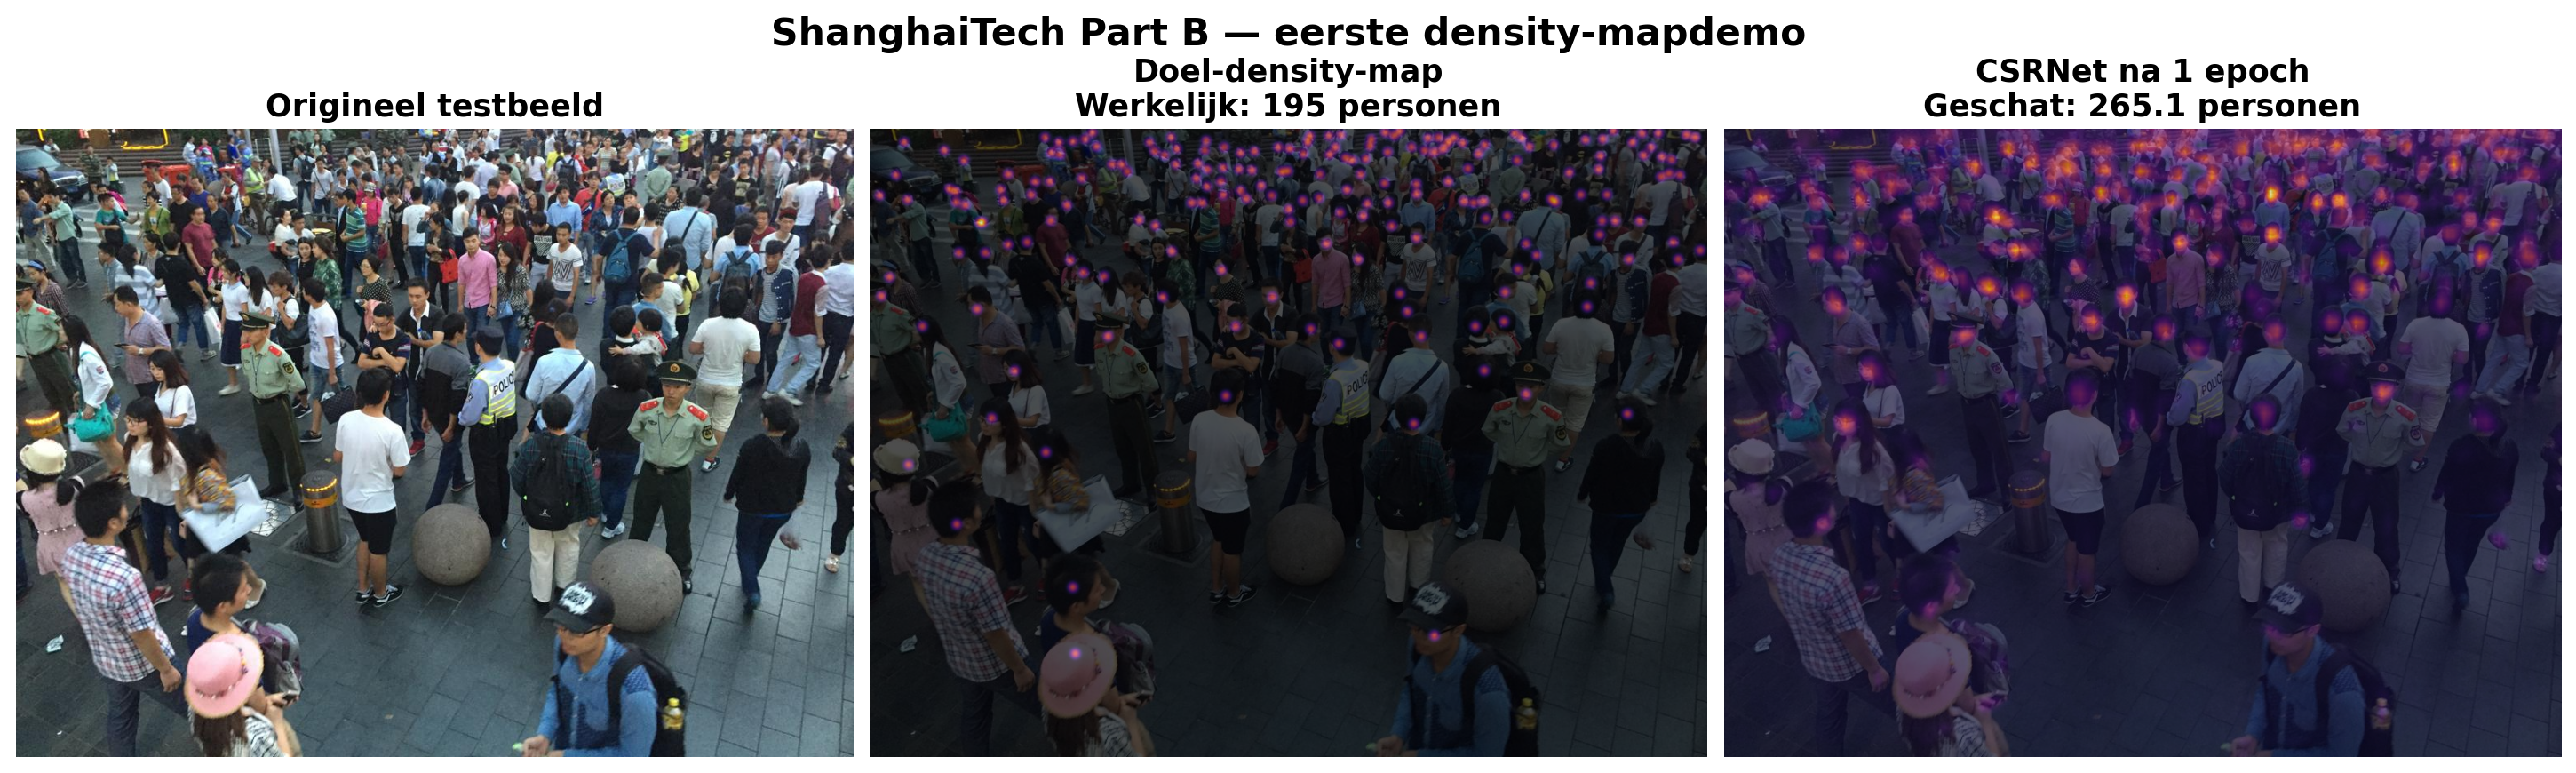
\includegraphics[width=\textwidth]{shanghaitech-density-map-vergelijking.png}
    \caption[Eerste density-mapvoorspelling]{Vergelijking tussen een origineel testbeeld, de density map op basis van de annotaties en de voorspelling van CSRNet na één epoch. De voorspelling lokaliseert een groot deel van de drukke zones, maar overschat de totale telling nog.}
    \label{fig:eerste-density-map}
\end{figure}

Deze meetwaarden zijn geen eindresultaat. Eén epoch is onvoldoende om CSRNet volledig te verfijnen, en de twee kalibratieruns verschillen in meer dan één instelling. Zij tonen wel aan dat de volledige keten werkt: ruwe puntannotaties worden omgezet naar density maps, de telling blijft behouden bij het schalen, het model kan worden getraind en de fout wordt op volledige beelden berekend. Een eerdere technische controle op centrale validatiecrops leverde een veel lagere fout op, maar bleek niet representatief voor de totale beeldtelling. Daarom wordt uitsluitend full-image-evaluatie behouden.

\subsection{Finale trainingsrun}

Na de kalibratie is CSRNet gedurende 100 epochs getraind volgens het vooraf vastgelegde protocol. De run gebruikt dezelfde 360 trainingsbeelden, 40 validatiebeelden, seed 42, cropgrootte van \(512 \times 512\) pixels, batchgrootte vier en leersnelheid \(10^{-5}\) als de gecontroleerde GPU-run van één epoch. Beide runs gebruiken dezelfde finale code en deterministische PyTorch-algoritmen. Ze registreren ook dezelfde hash van het datasetmanifest. Daardoor kan het verschil in tabel~\ref{tab:een-versus-honderd-epochs} als het effect van verdere training binnen deze ene configuratie worden gelezen. De officiële testset is niet voor deze vergelijking gebruikt.

\begin{table}[htbp]
    \centering
    \small
    \begin{tabular}{lrr}
        \toprule
        & \textbf{1 epoch} & \textbf{100 epochs} \\
        \midrule
        Geselecteerd checkpoint & epoch 1 & epoch 39 \\
        Trainingsloss geselecteerde epoch & \(7{,}1764\) & \(2{,}9051\) \\
        Validatie-MAE & \(27{,}946\) & \(6{,}556\) \\
        Validatie-RMSE & \(40{,}757\) & \(9{,}218\) \\
        Mediane absolute fout & \(20{,}134\) & \(3{,}789\) \\
        Gemiddelde getekende fout & \(-26{,}796\) & \(-0{,}304\) \\
        Gemiddelde model-inferentie & \(106{,}88\) ms & \(107{,}02\) ms \\
        Theoretische modeldoorvoer & \(9{,}356\) FPS & \(9{,}344\) FPS \\
        Totale duur van de run & ca. 27 s & \(58{,}19\) min \\
        \bottomrule
    \end{tabular}
    \caption[Vergelijking tussen één en 100 epochs]{Vergelijking op dezelfde vaste validatieset met dezelfde finale code en configuratie. Voor de run van 100 epochs wordt het vooraf geselecteerde checkpoint met de laagste validatie-MAE gerapporteerd.}
    \label{tab:een-versus-honderd-epochs}
\end{table}

De laagste validatie-MAE wordt bereikt op epoch 39. Tegenover de gecontroleerde run van één epoch daalt de MAE met \(76{,}5\%\) en de RMSE met \(77{,}4\%\). De gemiddelde getekende fout of bias verandert van een onderschatting met \(26{,}796\) personen naar een bijna neutrale waarde van \(-0{,}304\) personen. De gemiddelde modeltijd blijft vrijwel gelijk, zoals verwacht: het aantal getrainde epochs verandert de gewichten, maar niet de CSRNet-architectuur of het aantal bewerkingen tijdens een voorwaartse berekening. Op het beste checkpoint bedraagt de mediaan van de absolute fout \(3{,}789\) personen, het 95e percentiel \(18{,}232\) personen en de grootste absolute fout \(27{,}569\) personen.

\subsection{Inferentie op laptop en Raspberry Pi}

Naast de evaluatie op de laptop-GPU is dezelfde CSRNet-architectuur uitgevoerd op de Intel Core i7-12700H van de laptop en op een Raspberry Pi 5 Model B met 4 GB RAM. Voor de platformvergelijking verwerken alle systemen twintigmaal hetzelfde testbeeld van \(1024 \times 768\) pixels na drie opwarmruns. De CPU-metingen gebruiken het geselecteerde checkpoint van epoch 39. De beschikbare GPU-meting met dit exacte herhaalprotocol gebruikt het kalibratiecheckpoint van epoch 1. Dat checkpoint heeft andere gewichten, maar dezelfde architectuur, invoergrootte en hoeveelheid rekenwerk. De afzonderlijke evaluatie van het finale GPU-checkpoint over veertig validatiebeelden levert met \(107{,}02\) ms en \(9{,}344\) FPS vrijwel dezelfde doorvoer op.

\begin{table}[htbp]
    \centering
    \small
    \begin{tabular}{>{\raggedright\arraybackslash}p{3.1cm}rrrr}
        \toprule
        \textbf{Platform} & \textbf{Epoch} & \textbf{ms/beeld} & \textbf{FPS} & \textbf{Relatief t.o.v. Pi} \\
        \midrule
        RTX 3050 Ti laptop-GPU & 1 & \(109{,}16\) & \(9{,}161\) & \(100{,}3\times\) \\
        Core i7-12700H laptop-CPU & 39 & \(5267{,}09\) & \(0{,}190\) & \(2{,}1\times\) \\
        Raspberry Pi 5-CPU & 39 & \(10948{,}63\) & \(0{,}091\) & \(1{,}0\times\) \\
        \bottomrule
    \end{tabular}
    \caption[Inferentiesnelheid op drie platformen]{Gemiddelde tijd en theoretische modeldoorvoer voor CSRNet op één beeld van \(1024 \times 768\) pixels, na drie opwarmruns en over twintig gemeten runs. Alleen de voorwaartse modelberekening is gemeten.}
    \label{tab:inference-platforms}
\end{table}

\begin{figure}[htbp]
    \centering
    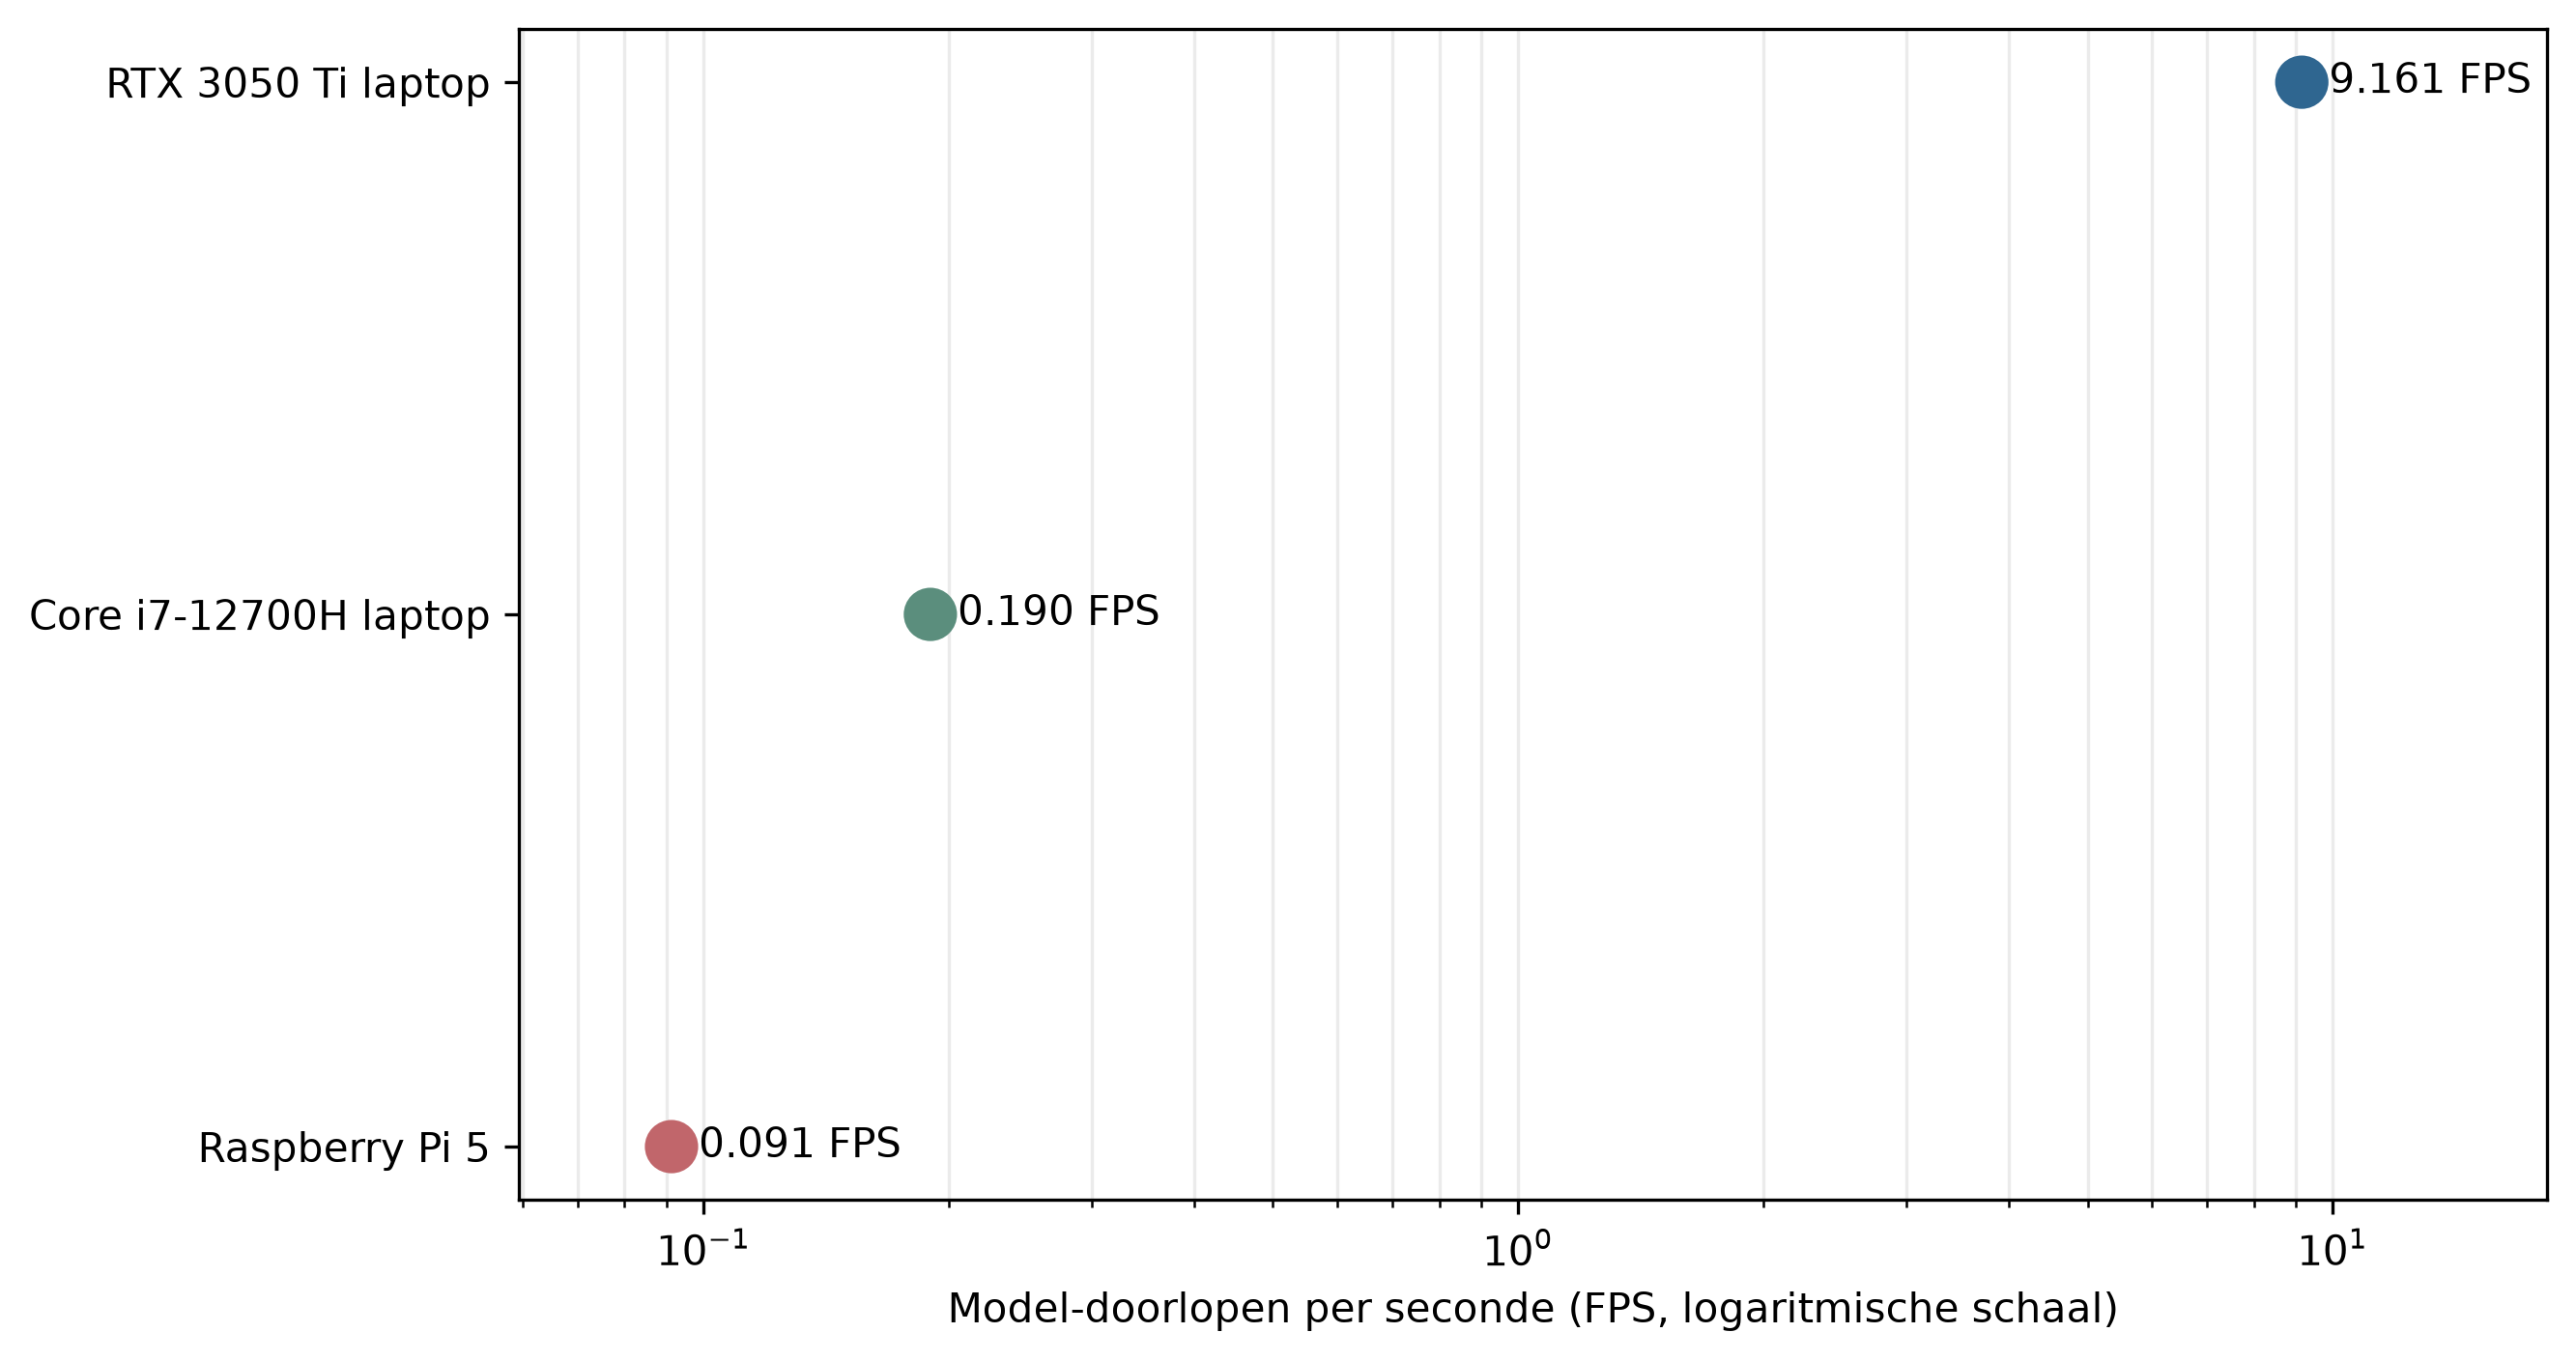
\includegraphics[width=0.92\textwidth]{csrnet-inference-platformvergelijking.png}
    \caption[CSRNet-modeldoorvoer per platform]{Modeldoorvoer per platform op een logaritmische schaal. De waarden zijn model-FPS en geen FPS van een volledige videoketen.}
    \label{fig:inference-platforms}
\end{figure}

De Raspberry Pi heeft gemiddeld \(10{,}95\) seconden nodig voor één beeld en haalt dus ongeveer één model-doorloop per elf seconden. De RTX 3050 Ti is in dit meetprotocol ongeveer honderdmaal sneller. Ook de laptop-CPU blijft met \(0{,}190\) FPS ruim onder de GPU. De identieke voorspelde telling van \(210{,}880\) personen op beide CPU's bevestigt dat hetzelfde checkpoint en dezelfde voorbewerking zijn gebruikt. Eén beeld zegt vanzelfsprekend niets over de nauwkeurigheid van het model op de volledige testset.

De Raspberry Pi startte de meetreeks bij \(57{,}9\)~\textdegree C en eindigde bij \(71{,}6\)~\textdegree C. Voor de test gaf \texttt{vcgencmd get\_throttled} de waarde \texttt{0x0}; nadien was dit \texttt{0xe0000}. Volgens de documentatie van Raspberry Pi betekenen de ingestelde historische bits dat frequentiebegrenzing, throttling en de zachte temperatuurlimiet tijdens de belasting zijn opgetreden \autocite{RaspberryPiVcgencmd}. Er was geen bit voor onderspanning ingesteld. De waarde van \(0{,}091\) FPS beschrijft daardoor het volgehouden gedrag met de aanwezige koeling, niet de korte piekprestatie van een koude processor.

Geen van de drie metingen haalt 15 FPS. Zelfs de laptop-GPU blijft met ongeveer \(9{,}3\) model-doorlopen per seconde onder die mogelijke doelwaarde, terwijl de volledige keten nog extra tijd vraagt. Ongewijzigde CSRNet-inferentie op de CPU van deze Raspberry Pi is dus niet bruikbaar voor een realtime videostroom. Een vervolgproef op edgehardware moet een lichter model, een kleinere invoerresolutie, pruning of kwantisatie onderzoeken en kan daarnaast een geschikte hardwareversneller testen.

Figuur~\ref{fig:csrnet-training-curves} toont het volledige trainingsverloop. De trainingsloss daalt globaal van \(7{,}1764\) op epoch 1 naar \(1{,}8015\) op epoch 100. De validatie-MAE en -RMSE fluctueren duidelijk, onder meer door de willekeurige trainingsuitsneden en de beperkte validatieset van veertig beelden. Er is geen eenduidig patroon van aanhoudende overfitting: ook na epoch 80 worden nog MAE-waarden tussen ongeveer zeven en negen bereikt. De laagste MAE ligt wel op epoch 39, waardoor het bewaren van \texttt{best.pt} noodzakelijk is en het laatste checkpoint niet automatisch als eindmodel mag worden gebruikt.

\begin{figure}[htbp]
    \centering
    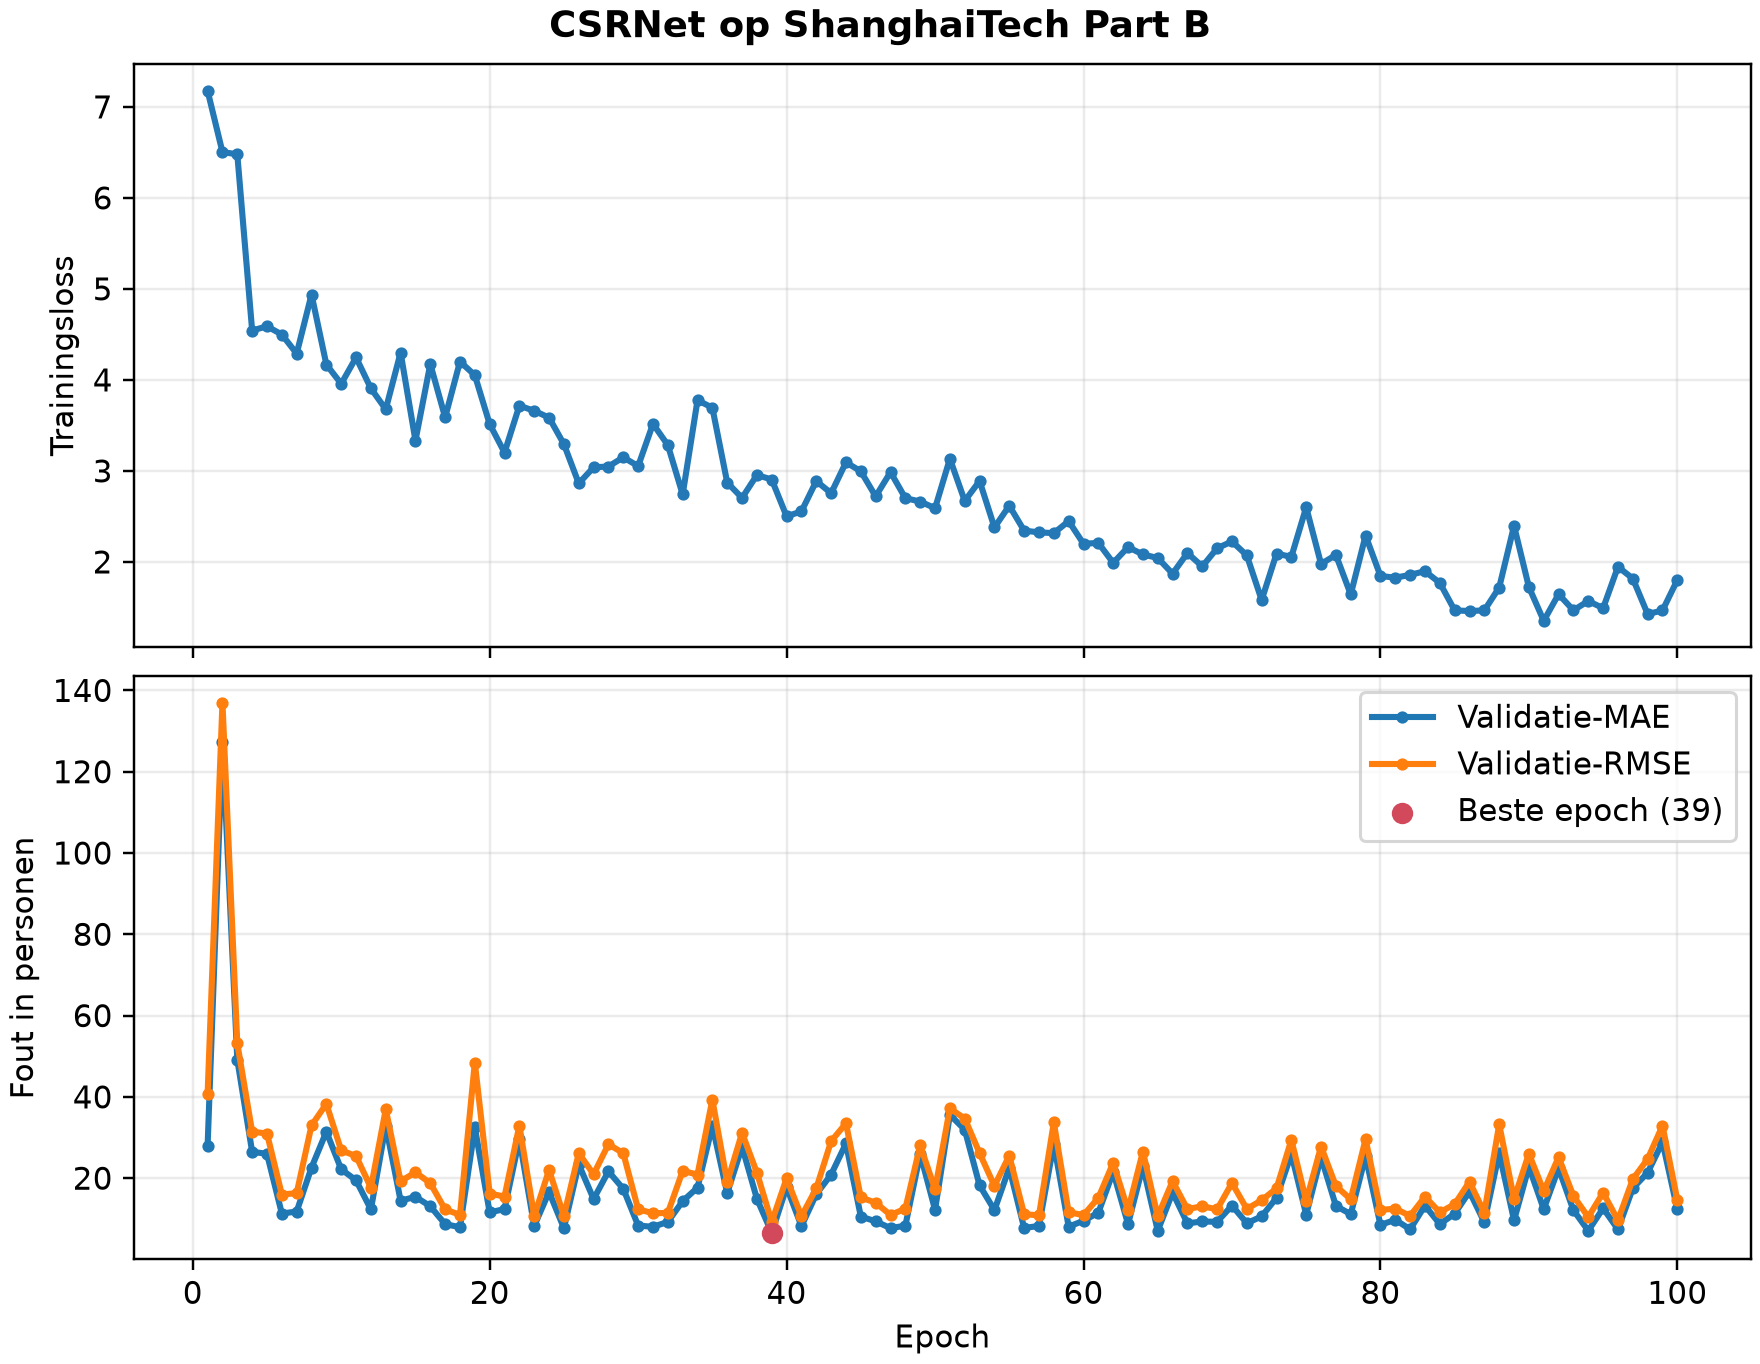
\includegraphics[width=0.9\textwidth]{csrnet-training-curves-100-epochs.png}
    \caption[Trainingsverloop van de finale CSRNet-run]{Trainingsloss en validatie-MAE/RMSE over 100 epochs. Het rode punt duidt de geselecteerde epoch 39 met de laagste validatie-MAE aan.}
    \label{fig:csrnet-training-curves}
\end{figure}

De run gebruikt bewust geen automatische early stopping, zodat het volledige verloop kan worden geanalyseerd. Het afzonderlijke beste checkpoint voorkomt dat latere, minder goede epochs het geselecteerde model vervangen. Voor bijkomende configuraties kan een vooraf vastgelegde patience worden toegevoegd om rekentijd te besparen, maar die keuze mag niet achteraf op basis van de testset worden aangepast.

De finale run bevestigt dat meerdere epochs noodzakelijk zijn om deze CSRNet-baseline te verfijnen. Voor een sterkere experimentele onderbouwing kunnen dezelfde configuratie met meerdere seeds en CSRNet met minstens één alternatief model, bijvoorbeeld MCNN, worden vergeleken. Daarna zijn rechtmatig verkregen beelden uit de doelcontext, camerakalibratie naar het grondvlak en een evaluatie per camera nodig. Pas dan kan worden beoordeeld in welke mate een model een bruikbare basis vormt voor druktemeting tijdens de Gentse Feesten.


% Voeg hier je eigen hoofdstukken toe die de ``corpus'' van je bachelorproef
% vormen. De structuur en titels hangen af van je eigen onderzoek. Je kan bv.
% elke fase in je onderzoek in een apart hoofdstuk bespreken.

%\input{...}
%\input{...}
%...

%%=============================================================================
%% Conclusie
%%=============================================================================

\chapter{Conclusie}%
\label{ch:conclusie}

Deze bachelorproef onderzocht hoe computervisie kan bijdragen aan tijdige indicaties van lokale drukte tijdens openluchtevenementen zoals de Gentse Feesten. De literatuurstudie toont dat lokale drukte niet uitsluitend door het aantal aanwezigen wordt bepaald. Ruimte, doorstroming, zichtbaarheid, de duur van een verhoogde bezetting en de samenwerking tussen diensten zijn eveneens bepalend. Een automatische meting kan menselijke observatie daarom ondersteunen, maar niet vervangen.

Voor dichte menigtes is density estimation een geschikte aanvulling op persoonsdetectie. Waar objectdetectie voor iedere persoon een afzonderlijk begrenzingskader moet vinden, voorspelt een density-estimationmodel een ruimtelijke verdeling en een totale telling. Daardoor is de methode beter bestand tegen overlap en schaalverschillen, al blijft zij afhankelijk van representatieve trainingsdata. CSRNet werd gekozen als eerste baseline omdat de architectuur voor dicht bezette scènes is ontworpen en op ShanghaiTech goed is gedocumenteerd.

De ontwikkelde PoC realiseert een reproduceerbare keten van puntannotaties naar density maps, training, full-image-validatie en visualisatie. Op ShanghaiTech Part B werd de officiële trainingsset met een vaste seed opgesplitst in 360 trainingsbeelden en 40 validatiebeelden. De officiële testset werd niet gebruikt voor modelselectie. In de finale GPU-run van 100 epochs ligt het checkpoint met de laagste validatie-MAE op epoch 39. Het behaalt een validatie-MAE van \(6{,}556\) personen, een RMSE van \(9{,}218\) personen en een bijna neutrale bias van \(-0{,}304\) personen. Tegenover een gecontroleerde run van één epoch met dezelfde configuratie dalen MAE en RMSE met respectievelijk \(76{,}5\%\) en \(77{,}4\%\). De volledige training duurt \(58{,}19\) minuten. Voor een beeld van \(1024 \times 768\) pixels bedraagt de gemiddelde tijd voor uitsluitend de voorwaartse modelberekening op de RTX 3050 Ti ongeveer \(107\) ms, of 9,3 FPS.

De centrale onderzoeksvraag kan bijgevolg als volgt worden beantwoord: computervisie kan met density estimation een bruikbare aanvullende indicatie geven van het geschatte aantal personen en van relatieve druktezones in een camerabeeld. Voor de Gentse Feesten is dat potentieel waardevol als één invoer voor een operator. De huidige PoC bewijst echter nog niet dat het systeem voldoende nauwkeurig, robuust of snel is voor operationeel gebruik. Met ongeveer 9,3 model-doorlopen per seconde voldoet de gemeten GPU-inferentie niet aan een eventuele doelwaarde van 15 beelden per seconde. Op de Raspberry Pi 5-CPU duurt één model-doorloop gemiddeld \(10{,}95\) s en wordt slechts \(0{,}091\) FPS bereikt. Daarbij trad thermische throttling op. Voor een beoordeling van real-timewerking moeten ook beeldopname, voorbewerking, visualisatie en communicatie worden gemeten.

Een cruciale beperking is het onderscheid tussen een density map en fysieke personendichtheid. De PoC werkt in beeldcoördinaten en kan zonder camerakalibratie, grondvlaktransformatie en afgebakende observatiezone geen waarde in personen per vierkante meter berekenen. Zij mag daarom geen zelfstandige alarmdrempel hanteren. Ook gebruikt ShanghaiTech Part B andere camerastandpunten en omgevingsomstandigheden dan de Gentse Feesten. Nachtelijke belichting, weersinvloeden, lokale architectuur en veranderende bezoekersstromen kunnen tot domeinverschuiving leiden. Representatieve, rechtmatig verkregen beelden uit de doelcontext zijn nodig om die generaliseerbaarheid te beoordelen.

Verder onderzoek moet de finale configuratie met meerdere seeds herhalen en CSRNet vergelijken met minstens één alternatief model, zoals MCNN. Ook de cropgrootte vraagt een gecontroleerde vergelijking. Uitsneden van bijvoorbeeld \(256\), \(384\), \(512\) en \(768\) pixels kunnen met dezelfde datasplit, hetzelfde aantal epochs en dezelfde overige hyperparameters worden getraind en op dezelfde volledige validatiebeelden worden beoordeeld. Zo kan worden nagegaan of extra beeldcontext de MAE en RMSE verbetert en hoeveel extra trainingstijd en GPU-geheugen dit kost. Vervolgens moeten de latentie van de volledige verwerkingsketen, het geheugenverbruik en de nauwkeurigheid per camera worden gemeten. Voor fysieke dichtheidsdrempels zijn per camera een kalibratie, een grondvlakprojectie en een validatieprocedure nodig. Ten slotte moet een reële uitrol worden aangevuld met gegevensbeschermingsmaatregelen, waaronder een duidelijke rechtsgrond, dataminimalisatie, beperkte bewaartermijnen en een beoordeling van de gegevensbescherming. Onder die voorwaarden kan de huidige PoC uitgroeien tot een geloofwaardige bouwsteen voor beslissingsondersteuning bij crowd management.


%---------- Bijlagen -----------------------------------------------------------

\appendix

\chapter{Onderzoeksvoorstel}

Het onderwerp van deze bachelorproef is gebaseerd op een onderzoeksvoorstel dat vooraf werd beoordeeld door de promotor. Dat voorstel is opgenomen in deze bijlage.

Het oorspronkelijke onderzoeksvoorstel vertrekt van de vraag hoe computervisie hulpdiensten en organisatoren kan ondersteunen met een actueel beeld van lokale drukte tijdens de Gentse Feesten. Het stelt voor om bestaande methoden voor crowd counting te onderzoeken en een Proof of Concept met density estimation uit te werken. De huidige bachelorproef verfijnt die ambitie: de PoC wordt uitsluitend beoordeeld als technische baseline op ShanghaiTech Part B. Zij levert een schatting van het aantal personen en relatieve druktezones in beeldcoördinaten, maar niet zonder bijkomende kalibratie een fysieke dichtheid in personen per vierkante meter of een operationeel alarm. De volgende pagina's bevatten het oorspronkelijke, vooraf beoordeelde voorstel.


% Verwijzing naar het bestand met de inhoud van het onderzoeksvoorstel
\input{../voorstel/voorstel-inhoud}

%%=============================================================================
%% Bijlage: broncode en reproduceerbaarheid
%%=============================================================================

\chapter{Broncode en reproduceerbaarheid}
\label{app:broncode}

Deze bijlage beperkt zich tot de code die de opbouw van CSRNet, de dataverwerking, de trainingslus en de inferentie bepaalt. Hulpscripts voor figuren, rapportage en regressietests zijn niet afgedrukt. De volledige uitvoerbare code staat in de volgende GitHub-repository:
\begin{center}
    \url{https://github.com/WouterVantienenHOGENT/bachelorproef}
\end{center}
De README bevat de commando's voor datavoorbereiding, training, evaluatie en inferentie.

De ruwe ShanghaiTech-data worden niet herverdeeld. Wie het experiment herhaalt, moet de dataset via de oorspronkelijke aanbieder verkrijgen. De digitaal ingediende runmappen bevatten de configuraties, metrieken en samenvattingen. Grote modelcheckpoints en de dataset maken geen deel uit van deze tekstuele bijlage.

\section{Pakketversies}

\subsection{Laptop-GPU}
\inputminted[fontsize=\scriptsize]{text}{../crowd_counting/requirements-final.txt}

\subsection{Raspberry Pi 5}
\inputminted[fontsize=\scriptsize]{text}{../crowd_counting/requirements-rpi.txt}

\clearpage
\section{CSRNet-model}
\inputminted[fontsize=\scriptsize]{python}{../crowd_counting/csrnet.py}

\clearpage
\section{Dataset en density maps}
\inputminted[fontsize=\scriptsize]{python}{../crowd_counting/data.py}

\clearpage
\section{Training}
Onderstaande fragmenten tonen de opbouw van de dataloaders en het model, gevolgd door de eigenlijke trainings- en validatielus. Argumentverwerking, hervatten van checkpoints en het wegschrijven van metriekbestanden zijn beschikbaar in het digitale bronbestand.
\begin{minted}[fontsize=\scriptsize,firstnumber=235]{python}
train_set = DensityMapDataset(
    args.train_images, args.train_densities, args.crop_size, "train"
)
val_set = DensityMapDataset(
    args.val_images, args.val_densities, args.crop_size, "eval"
)
loader_options = {
    "num_workers": args.workers,
    "pin_memory": device.type == "cuda",
    "generator": loader_generator,
}
train_loader = DataLoader(
    train_set,
    batch_size=args.batch_size,
    shuffle=True,
    **loader_options,
)
val_loader = DataLoader(
    val_set,
    batch_size=1,
    shuffle=False,
    **loader_options,
)

model = CSRNet(
    pretrained_frontend=not args.no_pretrained and resume_path is None
).to(device)
optimizer = torch.optim.Adam(model.parameters(), lr=args.lr, weight_decay=1e-4)
criterion = nn.MSELoss(reduction="sum")
scaler = torch.amp.GradScaler("cuda", enabled=device.type == "cuda")
\end{minted}

\begin{minted}[fontsize=\scriptsize,firstnumber=339]{python}
for epoch in range(start_epoch, args.epochs + 1):
    epoch_started = time.perf_counter()
    if device.type == "cuda":
        torch.cuda.reset_peak_memory_stats(device)
    model.train()
    running_loss = 0.0
    for images, targets, _ in train_loader:
        optimizer.zero_grad(set_to_none=True)
        with torch.autocast(
            device_type=device.type, enabled=device.type == "cuda"
        ):
            prediction = model(
                images.to(device, non_blocking=device.type == "cuda")
            )
            loss = criterion(
                prediction,
                targets.to(device, non_blocking=device.type == "cuda"),
            ) / images.shape[0]
        scaler.scale(loss).backward()
        scaler.step(optimizer)
        scaler.update()
        running_loss += loss.item()
    synchronize(device)
    training_seconds = time.perf_counter() - epoch_started

    validation_started = time.perf_counter()
    mae, rmse, forward_ms = evaluate(model, val_loader, device)
    validation_seconds = time.perf_counter() - validation_started
    epoch_seconds = time.perf_counter() - epoch_started
    train_loss = running_loss / len(train_loader)
    peak_memory_mib = (
        torch.cuda.max_memory_allocated(device) / (1024**2)
        if device.type == "cuda"
        else 0.0
    )
    metric: dict[str, object] = {
        "epoch": epoch,
        "train_loss": train_loss,
        "val_mae": mae,
        "val_rmse": rmse,
        "train_seconds": training_seconds,
        "validation_seconds": validation_seconds,
        "epoch_seconds": epoch_seconds,
        "val_forward_ms_per_image": forward_ms,
        "peak_cuda_memory_mib": peak_memory_mib,
        "completed_at_utc": utc_now(),
    }
    is_best = mae < best_mae
    if is_best:
        best_mae = mae
        best_metric = dict(metric)

    checkpoint = {
        "format_version": 2,
        "epoch": epoch,
        "model": model.state_dict(),
        "optimizer": optimizer.state_dict(),
        "scaler": scaler.state_dict(),
        "mae": mae,
        "rmse": rmse,
        "metric": metric,
        "best_metric": best_metric,
        "args": vars(args),
        "rng_state": capture_rng_state(loader_generator),
    }
    atomic_torch_save(checkpoint, output_dir / "last.pt")
    if is_best:
        atomic_torch_save(checkpoint, output_dir / "best.pt")
    if args.checkpoint_every and epoch % args.checkpoint_every == 0:
        atomic_torch_save(checkpoint, output_dir / f"epoch_{epoch:03d}.pt")
    append_metric(metrics_path, metric)
\end{minted}

\clearpage
\section{Inferentie en FPS-benchmark}
Dit fragment laadt een checkpoint en beeld, voert de opwarm- en meetruns uit en berekent de density map en model-FPS. De CLI-definitie en CSV-rapportage blijven in het digitale bronbestand.
\begin{minted}[fontsize=\scriptsize,firstnumber=65]{python}
device = select_device(args.device)
checkpoint = torch.load(args.checkpoint, map_location=device, weights_only=False)
model = CSRNet(pretrained_frontend=False).to(device)
model.load_state_dict(checkpoint["model"])
model.eval()
with Image.open(args.image) as source:
    image = source.convert("RGB")
array = np.asarray(image).copy()
tensor = torch.from_numpy(array).permute(2, 0, 1).float() / 255
tensor = (
    tensor - torch.tensor(IMAGENET_MEAN)[:, None, None]
) / torch.tensor(IMAGENET_STD)[:, None, None]
# Padding lets arbitrary image sizes pass through the stride-8 model.
pad_h, pad_w = (-image.height) % 8, (-image.width) % 8
tensor = F.pad(tensor, (0, pad_w, 0, pad_h)).unsqueeze(0).to(device)
with torch.inference_mode():
    for _ in range(args.warmup_runs):
        model(tensor)
    synchronize(device)
    forward_started = time.perf_counter()
    prediction = None
    for _ in range(args.timed_runs):
        prediction = model(tensor)
    synchronize(device)
    forward_seconds = time.perf_counter() - forward_started
    assert prediction is not None
    density = prediction[0, 0].cpu().numpy()
density = density[: (image.height + 7) // 8, : (image.width + 7) // 8]
output_dir = Path(args.output_dir)
output_dir.mkdir(parents=True, exist_ok=True)
stem = Path(args.image).stem
np.save(output_dir / f"{stem}_density.npy", density)
plt.imsave(output_dir / f"{stem}_density.png", density, cmap="jet")
forward_ms = 1000 * forward_seconds / args.timed_runs
frames_per_second = 1000 / forward_ms
\end{minted}


%%---------- Andere bijlagen --------------------------------------------------
% TODO: Voeg hier eventuele andere bijlagen toe. Bv. als je deze BP voor de
% tweede keer indient, een overzicht van de verbeteringen t.o.v. het origineel.
%\input{...}

%%---------- Backmatter, referentielijst ---------------------------------------

\backmatter{}

\setlength\bibitemsep{2pt} %% Add Some space between the bibliograpy entries
\printbibliography[heading=bibintoc]

\end{document}
